\documentclass[12pt]{scrartcl}
\usepackage[sexy]{evan}
\newcommand{\R}{\mathbb{R}}
\newcommand{\N}{\mathbb{N}}
\newcommand{\Q}{\mathbb{Q}}
\newcommand{\Z}{\mathbb{Z}}
\newcommand{\A}{\mathbb{A}}
\newcommand{\C}{\mathbb{C}}
\newcommand{\cF}{\mathcal{F}}
\newcommand{\bF}{\mathbb{F}}
\newcommand{\cO}{\mathcal{O}}
\newcommand{\pre}{^{-1}}
\newcommand{\maxideal}{\mathfrak{m}}
\newcommand{\primeideal}{\mathfrak{p}}

\usepackage{quiver}

\usepackage{relsize}
\begin{document}
\title{Note on Algebraic Geometry}
\author{Jiawen Huang}
\maketitle
\tableofcontents
\newpage
\section{Disclaimer}
This note is basically a copy of algebraic geometry note from Andreas Gathmann and algebraic geometry \href{https://www.youtube.com/playlist?list=PLn6dA-hP_G8SR-v8EV5m9vcpo-V9No-2V}{YouTube course} by Seidon Alsaody, Uppsala University. This note is written for my own reference. So there may be some typos and mistakes. Please kindly point them out to me if you find any.
\newpage 
\section{Preliminaries}
We assume our ground field $k$ is algebraically closed throughout the note.
\\
Preliminaries are basic abstract algebra. More specifically, you need to know 
\begin{itemize}
    \subsection{Basic abstract algebra}
    \item Rings
    \item Ideals: maximal, prime and radical ideals
    \item Fields and field extensions
    \item Noetherian Rings: three equivalent definitions and Hilbert's basis theorem. 
    \\

    {\LARGE{\textbf{Do not learn algebraic geometry if you are not comfortable with these concepts.}}}\\
\subsection{Affine Space and Affine Algebraic Sets}
    \item Affine Space $\A^n$: the set of all $n$-tuples of elements in $k$.
    \item Affine algebraic sets: $V(J)$ is the set of common zeros of all polynomials in $J$ or the set of common intersection of curve defined by polynomials in $J$. A subset of $\A^n$ is algebraic if it is of the form $V(J)$ for some ideal $J$ of $k[x_1,x_2,\ldots,x_n]$. 
    \item Algebraic sets of $\A^1$ must be finite sets or the whole set because a nonzero polynomial in one variable has only finite many roots. 
    \item Properties of $V(J)$:
    \begin{enumerate}
        \item If $I\subseteq J$, then $V(J)\subseteq V(I)$
        \item $V(I)\cap V(J)=V(I+J)$. More generally, $\bigcap_{\alpha} V(I_{\alpha})=V(\sum_{\alpha} I_{\alpha})$ (all but finitely many $I_{\alpha}$ are zero).
        \item $V(I)\cup V(J)=V(IJ)=V(I\cap J)$ (Nontrivial, notice that $IJ\subseteq I\cap J$. They are not equal in general. Exercise: If $I+J=R$ then $IJ=I\cap J$.) (This generalizes to finite union but not infinite union. Counterexample: the union of all points but one in $\A^1$ is not algebraic set.)
        \item $V(\sqrt{J})=V(J)$
    \end{enumerate}
\end{itemize}
\newpage 
\section{Hilbert's Nullstellensatz}
Let $A=k[x_1,x_2,\ldots,x_n]$ be the polynomial ring over an algebraically closed field $k$.
\begin{itemize}
    \item First, we need a reverse function of $V(J)$. Define $I(X)$ to be the ideal of $A$ consisting of all polynomials that vanish on $X\subseteq \A^n_k$. That is all the polynomials $f$ such that its curve passing through all points in $X$.
    \item Properties of $I(X)$:
    \begin{enumerate}
        \item If $X\subseteq Y$, then $I(Y)\subseteq I(X)$
        \item $I({a_1,a_2,\ldots,a_n})=(x_1-a_1,x_2-a_2,\ldots,x_n-a_n)$ (exercise, this is in fact not trivial)
        \item If $X$ is an algebraic set, then $V(I(X))=X$. (this is not hard)
    \end{enumerate}
    \item Nullstellensatz: For any ideal $J$ of $A$, $I(V(J))=\sqrt{J}$
    Proof sketch:
    \begin{enumerate}
    \item Zariski's Lemma: If $F$ is a finitely generated $k$-algebra that is also a field, then $F$ is a finite extension of $k$. There is an elementary proof if we assume $k$ is uncountable (Key: consider $\frac{1}{x-\lambda}$ for $\lambda\in k$ must be linearly dependent because $F$ is countable dimensional over $k$). We can use Noether normalization to prove this for general infinite $k$.
    \item Weak Version: $V(J)\neq \emptyset $ for all proper ideal $J$ of $A$. 
    \item Strong Version: Consider $J'=J+(1-fy)$ in $k[x_1,\ldots,x_n,y]$. 
    \end{enumerate}
    \item Some immediate consequences:
    \begin{enumerate}
        \item $I(X\cup Y)=I(X)\cap I(Y)$
        \item $I(X\cap Y)=\sqrt{I(X)+I(Y)}$
        \item If $f=g$ on $\A^n$, then $f=g$ in $A$.
        \item If $f_{\mid X}=g_{\mid X}$, then $(f-g)\in I(X)$. We say $f\equiv g \mod I(X)$.
    \end{enumerate}
\end{itemize}
\newpage 
\section{Regular Function on Closed Set}
Let $X\subseteq \A^n$ be an algebraic set. 
\begin{itemize}
    \subsection{Coordinate Rings}
    \item Definition: $\mathcal{O}(X)=\frac{k[x_1,x_2,\ldots, x_n]}{I(X)}$ is called the coordinate ring of $X$. This is clearly a $k$-algebra.
    \begin{example}
        $\mathcal{O}(\A^n)\cong A$
        \\
        $\mathcal{O}({p})\cong k$ (evaluation at point $p$)
        \\
        $\mathcal{O}(\ell)\cong k[t]$ where $\ell$ is a line in $\A^n$
    \end{example}
    \item A function $\phi$ on $X$ is called regular function or polynomial function if there exists $f\in A$ such that $\phi(x)=f(x)$ for all $x\in X$.
    \item There is a one-to-one correspondence between all the coordinate rings and all affine (affine means finitely generated) reduced $k$-algebras. Easy to show. 
\subsection{Algebraic Subset of $X$}
    \item Let $J$ be an ideal of $\mathcal{O}(X)$. Define $V_X(J)=\{p\in X\mid f(p)=0 \text{ for all } f \in J\}$. For any subset $Y$ of $X$, $Y$ is called an algebraic subset of $X$ if there exists an ideal $J$ of $\mathcal{O}(X)$ such that $Y=V_X(J)$.
    \item Let $\pi$ be the projection from $A$ to $\mathcal{O}(X)$. Notice that $V_X(J)$ is just $V(\pi^{-1}(J))$. So an algebraic subset of $X$ is also an algebraic set in $\A^n$.  
    \item We can also define $I_X(Y)=\{f\in \mathcal{O}(X)\mid f(p)=0 \text{ for all } p \in Y\}$. We can easily verify  $I_X(Y)=\frac{I(Y)}{I(X)}$.
    \item With this, we can easily verify the following properties:
    \begin{enumerate}
        \item $\mathcal{O}(Y)\cong \frac{\mathcal{O}(X)}{I_X(Y)}$
        \item We have the relative version of Nullstellensatz: For any ideal $J$ of $\mathcal{O}(X)$, $I_X(V_X(J))=\sqrt{J}$. (The proof is just applying the original Nullstellensatz and playing around with the quotient of ideals: $\frac{\sqrt{J}}{I(X)}=\sqrt{\frac{J}{I(X)}}$. More generally, the preimage of a radical ideal is radical) The weak one is also true: the maximal ideals of $\mathcal{O}(X)$ are in one-to-one correspondence the maximal ideals of $A$ that contains $I(X)$, which are in one-to-one correspondence with points in $X$.
    \end{enumerate}
    \begin{remark}
        Later on, we will just use $I$ and $V$ instead of $I_X$ and $V_X$ when there is no confusion (when the ground algebraic set $X$ is fixed).
    \end{remark}
\end{itemize}
\newpage
\section{Zariski's Topology}

\begin{itemize}
    \subsection{Basic Definitions}
    \item Definition: The closed sets of Zariski's topology on $\A^n$ are all the algebraic sets. 
    \begin{remark}
        The fact that algebraic sets form a topology is very surprising. 
    \end{remark}
    \item If $X$ is an algebraic set, we can define the Zariski's topology on $X$ similarly: closed sets are all the algebraic subsets of $X$ or the intersection of algebraic sets with $X$. (These two are the same)
    \item $\A^1$ is non-hausdorff, any nonempty open set is dense and has finite complement. In general, $\A^n$ is also non-hausdorff and any nonempty open set is dense (we will show it later).
    \subsection{Connectedness}
    \item An algebraic set $X$ is connected if we cannot write $X=X_1\cup X_2$ where $X_1, x_2$ are nonempty proper \textbf{disjoint} closed (closed under $X$ or $\A^n$, doesn't matter since $X$ itself is closed) subsets of $X$.
    \item Geometric intuition: connected means we can draw $X$ without lifting the pen.
    \item Algebraic perspective: If $X=X_1\cup X_2$ is disconnected, then $\mathcal{O}(X)\cong \mathcal{O}(X_1)\times \mathcal{O}(X_2)$ (this is just CRT)
    \item Some standard properties about connectedness: 
    \begin{enumerate}
        \item If a set $X$ admits an open connected covering $(U_i)$ such that $U_i\cap U_j\neq \emptyset$ for all $i,j$, then $X$ is connected. (exercise)
        \item Connectedness is preserved under continuous maps. 
        \item If $X$ is connected, so is $\overline{X}$. 
    \end{enumerate}
    \subsection{Irreducibility}
    \item An algebraic set $X$ is irreducible if we cannot write $X=X_1\cup X_2$ where $X_1, x_2$ are nonempty proper closed subsets of $X$. 
    \item Irreducibility implies connectedness but not vice versa (counterexample: $V(xy)$ in $\A^2$ is clearly connected but irreducible $V(xy)=V(x)\cup V(y)$.)
    \\
    \item Geometric intuition: irreducible means we cannot separate $X$ using "integral" several pieces. 
    \item We have discussed that open sets of $\A^n$ are very large. For example, nonempty open set of $\A^1$ is always dense. In fact, we have the following lemma to formalize and generalize this idea. 
    \begin{lemma}
        In any irreducible topological space $X$, any nonempty open set is dense in $X$. 
    \end{lemma}
    \begin{proof}
        Let $U$ be a nonempty open set in $X$. Consider $\overline{U}\cap (X-U)=\emptyset$. Thus, $\overline{U}=X$. (This proof is purely topological.)
    \end{proof}
    \begin{remark}
        Let $X$ be an irreducible algebraic set and $U$ be a nonempty open set of $X$. If $f=g$ on $U$, then $f=g$ on $X$. This is because $V_X(f-g)$ is closed in $X$ and contains $U$. Since $\overline{U}=X$, we have $X=\overline{U}\subseteq V_X(f-g)\subseteq X$. Thus, $f=g$ on $X$. This makes sense because open set is very large in irreducible algebraic set (dense).
    \end{remark}
    \item Algebraic perspective: $X$ is irreducible if and only if $\mathcal{O}(X)$ is an integral domain if and only if $I(X)$ is a prime ideal of $A$. 
    \\

    This is very nice! It allows us to study geometric irreducibility using algebraic tools: ideals and integral domains. With this characterization, we know all affine space $\A^n$ are irreducible just like $\A^1$. 
    \item Some standard properties about irreducibility:
    \begin{enumerate}
        \item Irreducibility is preserved under continuous maps. 
        \item A set is irreducible if and only if its closure is irreducible.
        \item If a set $X$ admits an open irreducible covering $(U_i)_{i\in I}$ such that $U_i\cap U_j\neq \emptyset$ for all $i,j$, then $X$ is irreducible. 
        \\
        Proof: Suppose $X=M\cap N$ where $M$ and $N$ are closed subsets of $X$, then consider $U_i=X\cap U_i=(M\cap U_i)\cup (N\cap U_i)$. Since $U_i$ is irreducible, we conclude that $U_i$ are either contained in $M$ or $N$. Assume $J\subset I$ such that $U_i\subseteq M$ for all $i\in J$ and $U_i\subseteq N$ for all $i\notin J$. Consider $M'=M\cap (X-\bigcup_{i\notin J} U_i)$ and $N'=N\cap (X-\bigcup_{i\in J} U_i)$. We have $X=M'\cup N'$ and $M'\cap N'=\emptyset$. So $X$ is disconnected unless one of $J=I$ or $J=\emptyset$. However, $X$ must be connected as we have shown before. Thus, $X$ is irreducible.
        \item If $X\subseteq \A^n$ is irreducible and $Y\subseteq \A^m$ is irreducible, then $X\times Y\subseteq \A^{n+m}$ is also irreducible. 
    \end{enumerate}
    \subsection{Noetherian Topological Space}
    \item A topological space $X$ is called Noetherian if every descending chain of closed subsets terminates. 
    \begin{corollary}
        Any algebraic set $X\subseteq \A^n$ is a Noetherian topological space. This follows from the fact that $k[x_1,x_2,\ldots,x_n]$ is a Noetherian ring, and its quotient $\mathcal{O}(X)$ is also Noetherian. 
    \end{corollary}
    There are six important properties of Noetherian topological spaces:
    \begin{enumerate}
    \item The subspace of a Noetherian topological space is also Noetherian. This is just like the submodule of a Noetherian module is also Noetherian. 
    \item Any Noetherian topological space can be decomposed into finite union of irreducible closed sets that are not contained in each other. This decomposition is unique up to permutation. 
    \\

    With this fact, we can more or less assume our ground algebraic set $X$ is irreducible because we can always decompose it into irreducible components.
    \item Similarly, any Noetherian topological space can be decomposed into finite \textbf{disjoint} union of connected closed sets that are not contained in each other. This decomposition is unique up to permutation. 
    \item If $X$ is the finite union of Noetherian topological spaces, then $X$ is also Noetherian.
    \item Noetherian is a topological property preserved under continuous maps.
    \item \textbf{A topological space $X$ is Noetherian if and only if every open subset of $X$ is compact if and only if every subspace of $X$ (induced topology from $X$)  is compact.} This is tremendous because compactness is a very useful property in topology. Anyway, the proof is an exercise. 
    \\

    This property makes sense because open sets are very large in Zariski's topology. So finite many open sets will be sufficient to cover an open set.
    \end{enumerate}
    \begin{remark}
        Noether killed infinite. Big thank you to Noether. 
    \end{remark}
    \subsection{Regular Function on Zariski's Open Set}
    Given a zariski's topology on an algebraic set $X$,
    \item We have defined the regular function on algebraic sets/closed set of $X$: coordinate rings. Now, we wish to define it on open set. So we may assume $X$ is an irreducible algebraic set, and we wish to define regular function on open set $U$ of Zariski's topology of $X$. 
    \\
    The problem is that $U$ is dense in $X$, so intuitively, $I(U)$ would be $0$ because $U$ is so large. Indeed, $V_X(I_X(U))=\overline{U}=X$ (this is true in general, $V(I(X))=\overline{X}$). So $I_X(U)=I_X(X)=0$. Alternative way to see this is that if $f$ vanishes on $U$, then $U\subseteq \overline{U}\subseteq V_X(f)\subseteq X$. So $f$ must be $0$. 
    \\
    Therefore, we can't define $\mathcal{O}_X(U)$ to be $\frac{\mathcal{O}(X)}{I_X(U)}$ because this is just $\mathcal{O}(X)$ again. Instead, we define it as follows:
    \item Definition: Let $X$ be an algebraic set and $U$ be a Zariski's open set of $X$. A function $f:U\to k$ is called a regular function on $U$ if for each point $p\in U$, there exists an open neighborhood $p\in U_p\subseteq U$ and $g,h\in \mathcal{O}(X)$ such that for all $q\in U_p$, $f(x)=\frac{g(x)}{h(x)}$ and $h(x)\neq 0$ for all $x\in U_p$. The set of all regular functions on $U$ is denoted by $\mathcal{O}(U)$. We can easily verify that $\mathcal{O}_X(U)$ (or just $\cO(U)$ if the grounded algebraic set $X$ is fixed) is a $k$-algebra.
    \begin{remark}
        The notion of regular function on open set may lead to some confusion because $X$ itself is an open set of $X$. So $\mathcal{O}(X)$ has two different meanings: the coordinate ring of $X$ and the set of regular functions on the open set $X$. In fact, they are the same! We will see this in remark 4.11. 
    \end{remark}
    
    \item We can also study the zero loci of a regular function on open set $U$. 
    \begin{lemma}
        $\phi\in \cO(U)$, then $V(\phi)=\{x\in U\mid \phi(x)=0\}$ is closed in $U$. 
    \end{lemma}
    \begin{proof}
        For any $p\in U$, we can write $\phi=\frac{g_p}{h_p}$ on some open neighborhood $U_p$ of $p$ where $g_p,h_p\in \mathcal{O}(X)$ and $h$ doesn't vanish on $U_p$. Consider $U_a\setminus V(\phi)=U_a\setminus V(g_p)$, which is open in $U_a$, thus open in $U$. So $U\setminus V(\phi)=\bigcup_{p\in U} (U_p\setminus V(\phi))$ is open in $U$. Therefore, $V(\phi)$ is closed in $U$.
    \end{proof}
    \begin{remark}
        A open set minus a closed set is still open. So this lemma is quite useful. 
    \end{remark}
    \begin{remark}[Identity Theorem of regular functions]
        With Lemma 4.6, we can see the following: If $X$ is irreducible algebraic set and $U\subseteq V$ are nonempty open sets of $X$, then if $\phi_1, \phi_2\in \mathcal{O}(V)$ and $\phi_{1\mid U}=\phi_{2\mid U}$, then $\phi_1=\phi_2$ on $V$. This is becasue $V(\phi_1-\phi_2)$ is closed in $V$ and contains $U$. Since $\overline{V}=X$, $V$ is irreducible. So $V=\overline{U}\subseteq V(\phi_1-\phi_2)\subseteq V$. This makes sense because open set is very large in irreducible algebraic set (dense). 
    \end{remark}
    \item The fact that the denominator depends on the choice of the point is quite annoying. It's a local definition. Here is an example: 
        \begin{example}
            Let $X=V(x_1x_4-x_2x_3)\subseteq \A^4$ and $U=X\setminus V(x_2,x_4)$. 
            Then, we have the following regular function on $U$:
            \[\phi=\begin{cases}
                \frac{x_1}{x_2} & \text{if } x_2\neq 0\\
                \frac{x_3}{x_4} & \text{if } x_4\neq 0
            \end{cases}\]
        This is clearly a regular function because it's locally a ratio of polynomials. But we can't write it globally as a ratio of polynomials. $k[x_1,x_2,x_3,x_4]/(x_1x_4-x_2x_3)$ is non UFD. 
        \end{example}
    \subsection{Regular function on principal open set}
    \item However, we can restrict our open set to be principal open set to have a global property. First, we define principal open set:
    \begin{definition}
        Let $X$ be an algebraic set and $f\in \mathcal{O}(X)$. Define $U_f=\{x\in X\mid f(x)\neq 0\}$. Then, $U_f$ is called the principal open set of $f$ in $X$.
    \end{definition}

    There are two basic properties of principal open sets:
    \begin{enumerate}
        \item The intersection of two principal open sets is also a principal open set because $U_f\cap U_g=U_{fg}$.
        \item Any open set $U$ of $X$ can be written as finite union of principal open sets. Trivial by Noetherian property.
    \end{enumerate}
    \item If $U_f$ is a principal open set of $f\in \cO(X)$, then we have a nice description of $\mathcal{O}(U_f)=\{\frac{g}{f^n}\mid g\in \mathcal{O}(X), n\in \mathbb{N}\}$. So we can write any regular function on $U_f$ as a ratio of polynomials with denominator being some power of $f$, something global.
    \begin{proof}
    Consider a regular function $\phi: U_f\to k$. For any $p\in U_f$, we have open set $U_p$ in $U_f$ such that $p\in U_p\subseteq U_f$ and $\phi=\frac{g}{h}$ for some $g, h\in \cO(X)$ and $h$ doesn't vanish on $U_p$. We may further assume $U_p=U_t$ for some $t\in \cO(X)$. The only thing we can do here is to multiply something on numerator and denominator to turn it into a better form. Consider $h'=h\cdot t$ and $g'=g\cdot t$. Then, we have $\phi=\frac{g'}{h'}$ on $U_p$. Notice that $h'$ doesn't vanish on $U_t$ but does vanish outside $U_t$. So $V(h')=V(t)$. So we may just assume $t=h'$. $g'$ also vanishes outside $U_t$. 
    \\

    Since $U_f$ is an open set in a Noetherian topological space, we have an finite open covering of $U_f$:
    \[U_f=\bigcup_{i=1}^m U_{h_i}\]
    Taking the complement we have: 
    \[V(f)=\bigcap_{i=1}^m V(h_i)\]
    By Nullstellensatz, we have some $n\in \mathbb{N}$ such that $f^n\in (h_1,h_2,\ldots,h_m)$. So there exists $a_i\in \cO(X)$ such that
    \[f^n=\sum_{i=1}^m a_i h_i\] 
    Now, consider the following: 
    \[\psi=\frac{\sum a_ig_i'}{\sum a_i h_i}\] 
    For any $p\in U_f$, for any $j$, if $p\in U_{h_j}$, then $\frac{a_jg_j'}{a_j h_j}$ is defined at $p$ and equals to $\phi(p)$. If $p\notin U_{h_j}$, then $h_j(p)=0$, so $g_j'(p)=0$ as well. So we can conclude $\psi(p)=\phi(p)$ (think about this step, look the first remark below). Therefore, $\psi=\phi$ on $U_f$. This shows that any regular function on $U_f$ can be written as $\frac{g}{f^n}$ for some $g\in \cO(X)$ and $n\in \mathbb{N}$. 
        
    \end{proof}
    \begin{remark}
        A key property about fraction is used here. If $\frac{a}{b}=\frac{c}{d}$, then $\frac{a}{b}=\frac{c}{d}=\frac{a+c}{b+d}$.
    \end{remark}
    \begin{remark}
    Let $f=1$. Then $U_f=X$. So we have $\mathcal{O}(X)=\{\frac{g}{1^n}\mid g\in \mathcal{O}(X), n\in \mathbb{N}\}=\mathcal{O}(X)$. This shows that the two different definitions of $\mathcal{O}(X)$ are indeed the same. 
    \end{remark}
    \begin{remark}
        This is clearly similar to localization of of $\cO(X)$ at the multiplicative set generated by $f$. In fact, they are isomorphic. Proof is easy but the result is somewhere remarkable. It tells us that two regular functions agrees on a principal open set $U_f$ if and only if they are equal as elements in the localization of $\cO(X)$ at $f$. This is the ultimate identity theorem of regular functions on principal open set including algebraic sets. 
    \end{remark}
    \item The regular functions on some non-principal open set may also be in a nice form. For example, we can consider $X=\A^2\setminus\{0\}$ (nothing special about the origin here, we can remove any point). We claim that $\cO(X)=k[x,y]$. 
    \begin{proof}
        Although $X$ is not a principal open set, we can write it as union of two principal open sets: $X=U_x\cap U_y$. 
        \\

        Any regular function on $U_x$ can be written as $\frac{f(x,y)}{x^n}$ for some $f\in k[x,y]$ and $n\in \mathbb{N}$. Similarly, any regular function on $U_y$ can be written as $\frac{g(x,y)}{y^m}$ for some $g\in k[x,y]$ and $m\in \mathbb{N}$. We assume $x\nmid f,g$ They must agree on $U_x\cap U_y=U_{xy}$, that is $f(x,y)y^m$ and $g(x,y)x^n$ agree on $U_{xy}$ Since $\A^2$ is irreducible, by identity theorem of regular functions, we have
        \[ f(x,y)y^m = g(x,y)x^n \text{ on } \A^2\]
        So \[f(x,y)y^m=g(x,y)x^n \text{ in } k[x,y]\]
        Since $k[x,y]$ is a UFD, we must have $x^n\mid f(x,y)$ and $y^m\mid g(x,y)$. Contradiction unless $n=m=0$. Therefore, any regular function on $X$ is actually a polynomial $f=g$ in $k[x,y]$. So $\cO(X)=k[x,y]$.
    \end{proof}
    \begin{remark}
        This is quite surprising because we have removed a point from $\A^2$ but the regular functions remain the same. This tells us that there is no rational function that is undefined only at one point in $\A^2$. This is not true if $k=\R$. Just consider $\frac{1}{x^2+y^2}$.
    \end{remark}
\end{itemize}
\newpage
\section{Presheaf and Sheaf }
\begin{itemize}
    \subsection{Presheaf and Sheaf}
    \item A presheaf $\cF$ of rings on a topological space $X$ is a contravariant functor from the topological space $X$ (a category with open sets as objects and inclusion as morphisms) to the category of rings. $\cF$ sends each open set of a ring $\cF(U)$ and each inclusion of open sets $V\subseteq U$ to a restriction ring homomorphism $\rho_{U,V}:\cF(U)\to \cF(V) : \phi_{\mid U} \mapsto \phi_{\mid V}$.
    \\
    For each open set $U\subseteq X$, the elements of $\cF(U)$ are called the sections of $\cF$ over $U$. 
    \\

    We also define $\cF(\emptyset)=0$ (the zero ring). This is just a convention, and it makes sense because $\emptyset$ is the initial object in the category of open sets of $X$ while $0$ is the final object in the category of rings. We can simply ignore this property in most situations.
    \\
    
    From on now, when we are discussing about sheaf on algebraic sets, 
    \begin{center}
        \fbox{we always assume any sheaf $\cF$ of rings is a sheaf of $k$-valued functions}
    \end{center}
   
    \item A sheaf is a presheat $\cF$ that satisfies the gluing property: 
    If $U\subseteq X$ is an open set, for any open covering of $U=\bigcup_{i\in I} U_i$, if we have $\phi_i\in \cF(U_i)$ such that ${\phi_i}_{\mid U_i\cap U_j}={\phi_j}_{\mid U_i\cap U_j}$ for all $i,j\in I$, then there exists a unqiue lift: that is a unique $\psi \in \cF(U)$ such that $\psi_{\mid U_i}=\phi_i$ for all $i\in I$.
    \begin{example}[Sheaf of Regular Functions]
        Let $X$ be an algebraic set with Zariski's topology. For any open set $U$, define $\cO_X(U)$ to be the set of all regular functions on $U$ for each open set $U\subseteq X$. Then $\cO_X$ is a sheaf of rings on $X$.
    \end{example}
    \begin{example}[Sheaf of Continuous Functions]
        Let $X$ be a subset of $\R^n$ with Euclidean topology. For any open set $U$, define $C^0(U,\R)$ to be the set of all continuous real-valued functions on $U$. Then $C^0(-,\R)$ is a sheaf of rings on $X$.
    \end{example}
    \begin{example}[A presheaf of constant functions, but not a sheaf]
        Let $X$ be a subset of $\R$ with Euclidean topology. For any open set $U$, define $C^{\text{constant}}(U,\R)$ to be the set of all constant real-valued functions on $U$. Then $C^{\text{constant}}(-,\R)$ is a presheaf of rings on $X$. But it's not a sheaf because the gluing of constant functions may not be constant. 
        \end{example}
    \begin{remark}
        The reason example 3 fails to be a sheaf is that the condition is global. In general, local conditions are easier to satisfy gluing condition. 
    \end{remark}

    \begin{remark}
        Intuitively, a presheaf on $U$, $\cF(U)$ is a set of functions defined on the open set $U$ of a topological space. This is why we say the presheaf \textbf{on} topological space $X$. And sheaf are presheaf such that the functions can be glued together nicely or define locally.
    \end{remark}
    \subsection{Stalks and germs}
    \item Let $\cF$ be a presheaf on a topological space $X$. For any point $p\in X$, we define the stalk of $\cF$ at $p$ to be the set \[\{(U,\phi)\mid \text{ open set }U\subseteq X, a\in U, \phi\in \cF(U) \}/\sim\]. $\sim$ is an equivalence relation defined as follows: $(U,\phi)\sim (V,\psi)$ if and only if there exists an open set $L \subseteq U\cap V$ such that $p\in L$ and $\phi_{\mid L}=\psi_{\mid L}$. The equivalence class of $(U,\phi)$ is called the germ of $\phi$ at $p$ and denoted by $\phi_p$. The stalk of $\cF$ at $p$ is denoted by $\cF_p$.
    \begin{remark}
        The germs in stalks are the function defined locally around the point $p$. So stalks capture the local behavior of the presheaf/sheaf at point $p$. The value at any point other than $p$ doesn't matter (we can always find a smaller neighborhood $U$ that doesn't contain that point).
    \end{remark}
    \begin{example}
        Consider the sheaf of differentiable functions on $\R$. The germs of a function $f$ at point $p$ captures the information about the value of $f$ at $p$ and all its derivative at $p$. 
    \end{example}
    \begin{example}
        Consider the sheaf of locally polynomial functions on $\R$. The stalk at point $p$ is isomorphic to the ring of $\R[x]$.
    \end{example}
    Next, we will see some basic properties of stalks in the sheaf of regular functions on algebraic sets.
    \item We denoted the stalk of the sheaf of regular functions $\cO_X$ at point $p$ by $\cO_{X,p}$. The most important information about $\cO_{X,p}$ is that it's isomorphic to the localization of the coordinate ring $\cO(X)$ at the maximal ideal $\maxideal_p$ corresponding to point $p$, \[\{\frac{f}{g}\mid f,g\in \cO(X), g(p)\neq 0\}\]. And it's a local ring with a unique maximal ideal $\maxideal_{X,p}=\{\phi_p\in \cO_{X,p}\mid \phi(p)=0\}$. The isomorphism is given by sending $\frac{g}{f}$ in the localization $\cO(X)_{\maxideal_p}$ to $(U_f, \frac{g}{f})$ in the stalk $\cO_{X,p}$. 
    \begin{remark}
        An algebraic fact about local rings: A ring is a local ring if and only if the set of non-unit elements forms an ideal. In our case, the set of non-unit elements is exactly $\maxideal_{X,p}$.
    \end{remark}
    \end{itemize}
\newpage
\section{Ringed Spaces and its morphisms}
\begin{itemize}
    \subsection{Ringed Space and Affine Varieties}
    \item A ringed space is a topological space $X$ equiped with a sheaf of rings $\cO_X$ on $X$. The sheaf $\cO_X$ is called the structure sheaf of the ringed space $(X,\cO_X)$.
    \item If $U$ is an open set of a ringed space $(X,\cO_X)$, then $(U,\cO_{X\mid U})$ is also a ringed space where $\cO_{X\mid U}$ is the restriction of $\cO_X$ on $U$, which is also a sheaf. ($\cO_{X\mid U}(V):=\cO_x(V)$ for all open set $V\subseteq U$)
    \item An affine variety is a ringed space that is \textbf{isomorphic as ringed space} to $(X,\cO_X)$ for some algebraic set $X$ with Zariski's topology and $\cO_X$ is the sheaf of regular functions on $X$.
    \item Well, what is the morphism of ringed space? 
    \item First of all, ringed spaces are topological spaces so we need the morphism to be some kind of continuous map $f$ from $X$ to $Y$. 
    \item Next, we need $f$ to preserve the sheaf structure or compatible with the sheaf functor. 
    \\
    For any open set $U\subseteq Y$, by continuity, we know that $U$ comes from the open set $f^{-1}(U)$. So we wish the function from $f^{-1}(U)$ to $k$ defined by $f^{*}(\phi)=\phi\circ f$ to be a section in $\cO_X(f^{-1}(U))$. In other words, we define the pullback of a section $\phi \in \cO_Y(U)$ as a function from $f^{-1}(U)$ to $k$ defined by $f^{*}(\phi)=\phi\circ f$. A morphism of ringed spaces is a continuous map from $X$ to $Y$ such that $f^{*}(\phi)$ to be a section in $\cO_X(f^{-1}(U))$ for any open set $U\subseteq Y$.
    \\

    Then, a morphism of ringed spaces from $(X,\cO_X)$ to $(Y,\cO_Y)$ is a continuous map $f:X\to Y$ such that for any open set $U\subseteq Y$ and any section $\phi \in \cO_Y(U)$, the pullback $f^{*}(\phi)\in \cO_X(f^{-1}(U))$.
    \item Properties of morphisms of ringed spaces:
    \begin{enumerate}
        \item The composition of two morphisms of ringed spaces is still a morphism of ringed spaces. And the identity is also a morphism of ringed spaces. So we can form a category with ringed spaces as objects and morphisms of ringed spaces as morphisms.
        \item If $f$ is a morphism from $(X,\cO_X)$ to $(Y,\cO_Y)$, let $U\subseteq X$ and $V\subseteq Y$ be an open sets such that $f(U)\subseteq V$, then $f_{\mid U}$ is a morphism of ringed spaces from $(U,\cO_{X\mid U})$ to $(V,\cO_{Y\mid V})$.
        \item Converse to 2, if for any open covering $(U_i)$ of $X$, $f_{\mid U_i}$ is a morphism of ringed spaces from $(U_i,\cO_{X\mid U_i})$ to $(Y,\cO_Y)$, then $f$ is a morphism of ringed spaces from $(X,\cO_X)$ to $(Y,\cO_Y)$. 
        \begin{proof}
            For any open set $V\subseteq Y$ and any section $\phi\in \cO_Y(V)$, 
            \[f^{*}(\phi)_{\mid U_i\cap f^{-1}(V)}=\phi\circ f_{\mid U_i}\in \cO_X(U_i\cap f^{-1}(V)).\] By the gluing property of sheaf, we have $f^{*}(\phi)\in \cO_X(f^{-1}(V))$. Therefore, $f$ is a morphism of ringed spaces.
        \end{proof}
    \end{enumerate}
    \item An isomorphism of ringed spaces is a morphism of ringed spaces that admits an inverse morphism of ringed spaces. (Just like homeomorphism in topology) 
    \begin{example}[Bijective morphism is not isomorphism]
        Consider the map from $\A^1$ to $V(y^2-x^3)\subseteq \A^2$ defined by $t\mapsto (t^2,t^3)$. This is a bijective morphism of ringed spaces but not an isomorphism of ringed spaces because the inverse map is not a morphism of ringed spaces. 
        \\
        
        But why? How do we show it's not a morphism of ringed spaces? Motivated by this question, we need a more concrete description of morphisms of ringed spaces between affine varieties.
    \end{example}
    \item The morphisms on affine varieties are the morphisms of ringed spaces between them. But we can describe them more explicitly:
   \begin{theorem}
    If $X\subseteq \A^n$ and $Y\subseteq \A^m$ are algebraic sets. For any open set $U\subseteq X$, if $f$ is a morphism from $(U,\cO_{X\mid U})$ to $(Y,\cO_Y)$, then $f=(f_1,f_2,\ldots, f_n)$ such that $f_1, f_2, \ldots, f_n\in \cO_{X\mid U}(U)=\cO_X(U)$. 
    \end{theorem}
    \begin{proof}
        If $f:U\to Y$ is a morphism, consider $V=Y$ and $y_i\in \cO_Y(Y)$. $f^*y_i=y_i\circ f=f_i\in \cO_X(f\pre(Y))=\cO_X(U)$. 
        \\
        Conversely, if $f=(f_1,f_2,\ldots, f_n)$ such that $f_i\in \cO_X(U)$, for any open set $V\subseteq Y$ and any section $\phi\in \cO_Y(V)$, we have $f^*\phi=\phi\circ f=\phi(f_1,f_2,\ldots, f_n)\in \cO_X(U)$ because regular functions are closed under composition. Therefore, $f$ is a morphism of ringed spaces.
    \end{proof}
    \item With the explicit description of morphisms of ringed spaces between affine varieties, we can link the morphisms of ringed spaces to the homomorphisms of their coordinate rings:
    \begin{theorem}
        There is a one-to-one correspondence between the morphisms of ringed spaces from $(X,\cO_X)$ to $(Y,\cO_Y)$ and the $k$-algebra homomorphisms from $\cO(Y)$ to $\cO(X)$.
    \end{theorem}
    \begin{proof}
        Given a morphism of ringed spaces $f:(X,\cO_X)\to (Y,\cO_Y)$, $f^*$ is a $k$-algebra homomorphism from $\cO(Y)$ to $\cO(X)$.
        \\

        Now, we construct its inverse map. Given a $k$-algebra homomorphism $g:\cO(Y)\to \cO(X)$, we define a function $f$ from $X$ to $\A^m$ (the ambient space of $Y$) as follows: 
        \[f=(g(y_1), g(y_2), \ldots, g(y_m))\]
        If the range of $f$ is contained in $Y$, by the theorem above, $f$ is a morphism of ringed spaces from $(X,\cO_X)$ to $(Y,\cO_Y)$.
        \\
        Now, we show that the image of $f$ is contained in $Y$. To show this, by Nullstellensatz, we need to show $I(im(f))\supseteq I(Y)$. For any $h\in I(Y)$, we have $g(h)=g(0)=0$ in $\cO(X)$. So $g(h)=h\circ f=0$ on $X$. Thus, $h$ vanishes on $im(f)$. Therefore, $I(im(f))\supseteq I(Y)$ and $im(f)\subseteq Y$. 
        \\
        Finally, we can easily verify that these two maps are inverses of each other.
    \end{proof}
    \begin{remark}
        This theorem is very important because it allows us to study geometric morphisms using algebraic homomorphisms. Beyond that, it shows that the category of affine varieties is (contravariantly) equivalent to the category of finitely generated reduced $k$-algebras. 
        \\
        This gives us a powerful tool to see if two affine varieties are isomorphic or not by checking if their coordinate rings are isomorphic or not.
    \end{remark}
    \item Now, we can come back to the example above. The map from $\A^1$ to $V(y^2-x^3)\subseteq \A^2$ defined by $t\mapsto (t^2,t^3)$ is not an isomorphism of ringed spaces. It's clearly that it's a bijective morphism of ringed spaces. However, if it's an isomorphism, then $\cO(V(y^2-x^3))\cong \frac{k[x,y]}{(y^2-x^3)}$ must be isomorphic to $\cO(\A^1)=k[t]$ under the map $x\mapsto to t^2$ and $y\mapsto t^3$. But $\cO(V(y^2-x^3))=k[x,y]/(y^2-x^3)$ is not isomorphic to $k[t]$ because $k[x,y]/(y^2-x^3)$ is not a UFD while $k[t]$ is a UFD. Therefore, the map is not an isomorphism of ringed spaces.
    \subsection{Product of affine Varieties}
    \item We wish to define the product of two affine varieties $X\subseteq \A^n$ and $Y\subseteq \A^m$. First of all, the product needs to be a topological space. So we may consider $X\times Y$ with the product topology (open sets are generated by $U\times V$ where $U$ is open in $X$ and $V$ is open in $Y$). However, this has some problem: 
    \begin{example}
        $V(x-y)\subseteq \A^2$ is closed in $\A^2$ with Zariski's topology. However, if we consider $\A^1\times \A^1$ with product topology, then $V(x-y)$ is not closed. (Exercise)
    \end{example}
    \item Therefore, we need to define a better topology on $X\times Y$. In fact, we can define a Zariski's topology on $X\times Y$ because $X\times Y$ is a closed subset of $\A^{n+m}$! 
    \item We can verify that this definition of topology on $X\times Y$ satisfies the universal property of product in the category of ringed spaces. 
\[\begin{tikzcd}
	Z \\
	\\
	&& {X\times Y} && X \\
	\\
	&& Y
	\arrow["f"', from=1-1, to=3-3]
	\arrow["{f_X}"', from=1-1, to=3-5]
	\arrow["{f_Y}", from=1-1, to=5-3]
	\arrow["{\pi_X}", from=3-3, to=3-5]
	\arrow["{\pi_Y}"', from=3-3, to=5-3]
\end{tikzcd}\]
We can apply our functor $\cO_{-}$ to get the following diagram in the category of $k$-algebras:
\[\begin{tikzcd}
	{\mathcal{O}(Z)} \\
	\\
	&& {\mathcal{O}(X\times Y)} && {\mathcal{O}(X)} \\
	\\
	&& {\mathcal{O}(Y)}
	\arrow["{f^*}", from=3-3, to=1-1]
	\arrow["{f_X^*}"', from=3-5, to=1-1]
	\arrow["{\pi_X^*}"', from=3-5, to=3-3]
	\arrow["{f_Y^*}", from=5-3, to=1-1]
	\arrow["{\pi_Y^*}", from=5-3, to=3-3]
\end{tikzcd}\]
So $\cO(X\times Y)$ satisfies the universal property of tensor product in the category of $k$-algebras. Since the functor $\cO_{-}$ is an equivalence of categories between the category of affine varieties and the category of finitely generated reduced $k$-algebras, we have:
\[\mathcal{O}(X\times Y)\cong \mathcal{O}(X)\otimes_k \mathcal{O}(Y)\]
\subsection{Some strange affine varieties }
\item In fact, affine varieties don't have to be algebraic sets. 
\begin{example}
    Principal open set $U_f$ of an algebraic set $X$ can be seen as an affine variety. 
    \\
    Let $Y:=\{(x,t)\in U_f\times \A^1 \mid tf(x)=1\} \subseteq \A^{n+1}$. Then, $(Y,\cO_Y)$ is an affine variety, and it's isomorphic to $(U_f,\cO_{X\mid U_f})$ as ringed space via the projection map $\pi:X\to U_f$. The inverse map is given by $x\mapsto (x, \frac{1}{f(x)})$. 
    \\
    The coordinate ring of $Y$ is given by:
    \[\mathcal{O}(Y)\cong \frac{\mathcal{O}(X)[t]}{(tf-1)}\cong \mathcal{O}(X)_f\]
    
\end{example}
\begin{example}[$\A^2\setminus \{0\}$ is not an affine Varieties]
    This is clear because we have shown that the regular functions on $\A^2\setminus \{0\}$ is $k[x,y]$. If it's an affine variety, then its coordinate ring must be isomorphic to $k[x,y]$. So $\A^2\setminus \{0\}$ must be isomorphic to $\A^2$ as ringed spaces, clearly a contradiction.
\end{example}
\end{itemize}
\newpage

% \section{Tools from Commutative Algebra that we need (to be finished)}
% Since this is an algebraic geometry note, we omit all the proofs in this section. 
% \begin{itemize}
%     \subsection{Integral extension}
%     \item This is the analog of algebraic extension in field theory. The idea is to make the extension $R'$ of $R$ a finitely generated module over $R$. 
%     \begin{definition}
%         Let $R\subseteq R'$ be an extension of rings. An element $r'\in R'$ is said to be integral over $R$ if there exists a monic polynomial $f(x)\in R[x]$ such that $f(r')=0$. The extension $R\subseteq R'$ is called an integral extension if every element of $R'$ is integral over $R$.
%     \end{definition}
%     \begin{theorem}
%         If $R\subseteq R'$ is an extension of rings and $R'=R[a_1, \ldots, a_n]$ is a finitely generated $R$-algebra, then the following are equivalent:
%         \begin{enumerate}
%             \item $R\subseteq R'$ is an integral extension.
%             \item Each $a_i$ is integral over $R$.
%             \item $R'$ is a finitely generated $R$-module.
%         \end{enumerate}
%             The proof requires the Cayley-Hamilton theorem to construct the characteristic polynomial to be the monic polynomial. This is also called the determinant trick. 
%     \end{theorem}
%     \begin{example}
%         $R=\C[x]$ and $R'=\C[x,y]/(y^2-x^2)$. Then, $R\subseteq R'$ is an integral extension because $y$ is integral over $R$ as it satisfies the monic polynomial $y^2-x^2=0$.
        
%         There is a geometric interpretation of this example. The ring inclusion $R \to R'$ corresponds to a morphism of affine varieties from $V(y^2-x^2)$ to $\A^1$ defined by $(x,y)\mapsto x$. 
%         \begin{center}
%             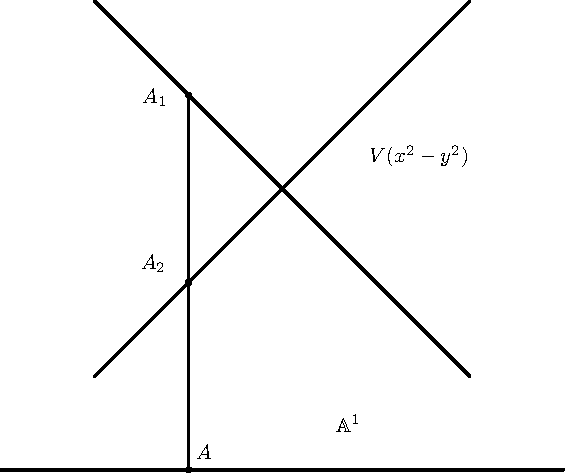
\includegraphics{diagram1-1.pdf}
%         \end{center}
        
%     The geometric meaning of integral extension is that for any point $A\in \A^1$, the preimage of $A$ under this morphism consists of finitely many points (in this case, only 2 points $A_1$ and $A_2$ are the preimage of $A$). 
%     \end{example}
%     \begin{example}[Non integral extension]
%         $R=\C[x]$ and $R'=\C[x,y]/(yx-1)$. This is not an integral extension because $y$ is not integral over $R$ as there is no monic polynomial in $R[x]$ that $y$ satisfies.
        
%         Geometrically, the ring inclusion $R \to R'$ corresponds to a morphism of affine varieties from $V(yx-1)$ to $\A^1$ defined by $(x,y)\mapsto x$.
%         \begin{center}
%             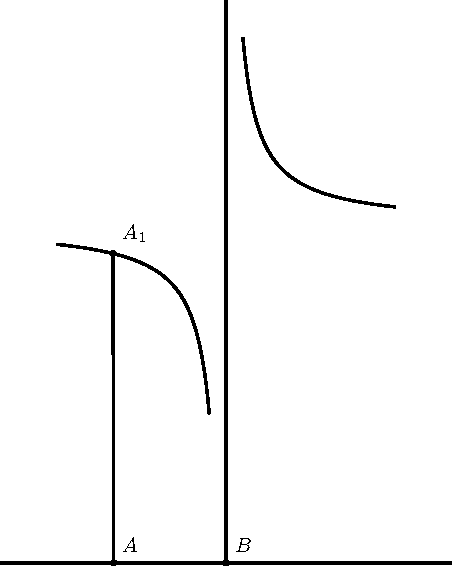
\includegraphics{diagram1-2.pdf}
%         \end{center}
%     The geometric meaning of non-integral extension is that there exists a point $B\in \A^1$ such that the preimage of $B$ under this morphism is an \textbf{infinite set} or an \textbf{empty}. 
%     \end{example}
%     \begin{example}[Non integral extension]
%         $R=\C[x]$ and $R'=\C[x,y]/(xy)$.
%         \begin{center}
%             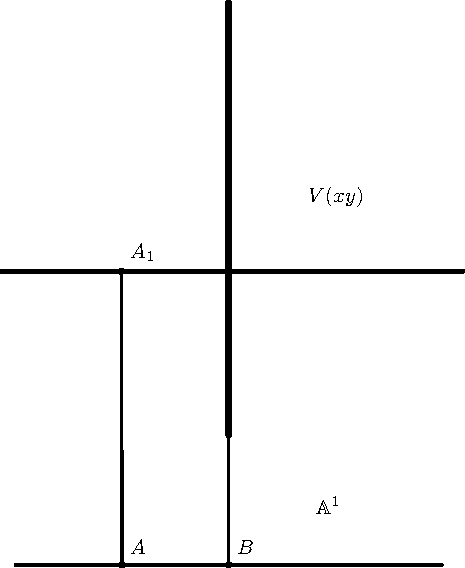
\includegraphics{diagram1-3.pdf}
%         \end{center}
%         The preimage of $B=0$ is infinite. 
%     \end{example}

% \end{itemize}

\section{Prevarieties and Varieties}
\subsection{Constructing Prevarieties}
The problem with affine varieties is that not all "nice" spaces are affine varieties. For example, $\A^2\setminus \{0\}$ is not an affine variety. So we need to generalize the notion of affine varieties to include more "nice" spaces. This leads us to the notion of prevarieties and varieties. 

\begin{definition}
    A prevariety is a ringed space $X$ such that $X$ can be covered by finitely many open sets $U_i\subseteq X$ such that each $(U_i, \cO_{X\mid U_i})$ is an affine variety (that is isomorphic to some $(Y,\SO_Y)$ for some algebraic set $Y$ as ringed space). $U_i$ are called affine open sets of the prevariety $X$. Morphisms of prevarieties are defined to be morphisms of ringed spaces.
\end{definition}
\begin{remark}
    The open cover is not part of the data of prevariety. The existence of different finite open cover by affine varieties leads to the same prevarieties if prevarieties are isomorphic as ringed spaces.
\end{remark}
\begin{remark}
    It's clear that any affine variety is a prevariety. Moreover, any open set of a affine variety is a prevariety because any open set of an affine variety can be covered by finitely many principal open sets, which are all affine varieties. 
    \\

    Moreover, any open subset of a prevariety is also a prevariety because we can cover it with the open subsets of the affine open sets which can be covered by finitely many affine varieties. The sheaf structure on the open subset is just the restriction of the sheaf structure on the prevariety. This is called the open subprevariety of a prevariety.
    \\

    We can also define the closed subprevariety of a prevariety $X$. We will do this later. 
\end{remark}

The basic way to construct prevarieties is to glue affine varieties together or to glue finitely many prevarieties. Let's first glue two prevarieties together $(X_1, \SO_{X_1})$ and $(X_2, \SO_{X_2})$. Let $U_{12}\subseteq X_1$ and $U_{21}\subseteq X_2$ be open sets such that there exists an isomorphism of ringed spaces $f_{12}:U_{12}\to U_{21}$. Therefore, we can glue $X_1$ and $X_2$ together along $U_{12}$ and $U_{21}$ via $f_{12}$.
More precisely, 
\begin{itemize}
    \item As a set, we define $X=(X_1\sqcup X_2)/\sim$ where $\sim$ is the equivalence relation defined as follows: $a\sim b$ if $a=b$ or $a\in U_{12}, b\in U_{21}$ and $f_{12}(a)=b$ or the other way around.
    \item As a topological space, we first define the topological space on $X_1\sqcup X_2$ to be the coproduct of topological spaces $X_1$ and $X_2$, that is the finest topological space such that the inclusion maps $i_1':X_1\to X_1\sqcup X_2$ and $i_2':X_2\to X_1\sqcup X_2$ are continuous. Next, we define the topology on $X$ to be the quotient topology induced by the quotient map $\pi:X_1\sqcup X_2\to X$, that is the finest topology on $X$ such that $\pi$ is continuous. 
    % https://q.uiver.app/#q=WzAsNCxbMSwxLCJYXzFcXHNxY3VwIFhfMiJdLFswLDAsIlhfMSJdLFswLDIsIlhfMiJdLFszLDEsIlg9WF8xXFxzcWN1cCBYXzIvXFxzaW0iXSxbMSwwLCJpXzEnIl0sWzIsMCwiaV8yJyIsMl0sWzAsMywiXFxwaSIsMl0sWzEsMywiaV8xIiwxLHsiY3VydmUiOi0yfV0sWzIsMywiaV8yIiwxLHsiY3VydmUiOjJ9XV0=
\[\begin{tikzcd}
	{X_1} \\
	& {X_1\sqcup X_2} && {X=(X_1\sqcup X_2)/\sim} \\
	{X_2}
	\arrow["{i_1'}", from=1-1, to=2-2]
	\arrow["{i_1}"{description}, curve={height=-12pt}, from=1-1, to=2-4]
	\arrow["\pi"', from=2-2, to=2-4]
	\arrow["{i_2'}"', from=3-1, to=2-2]
	\arrow["{i_2}"{description}, curve={height=12pt}, from=3-1, to=2-4]
\end{tikzcd}\]
    Therefore, $U\subseteq X$ is open if and only if $i_1^{-1}(U)$ is open in $X_1$ and $i_2^{-1}(U)$ is open in $X_2$. 
    \item As a ringed space, for any open set $U\subseteq X$, we define
    \[\SO_X(U):=\{\phi: U\to K\mid i_1^*\phi \in \SO_{X_1}(i_1^{-1}(U))\text{ and }i_2^*\phi \in \SO_{X_2}(i_2^{-1}(U))\}\]
 
    This definition is motiavted by universal construction, this is the largest/finest sheaf (largest number of $\phi$ such that $i_1$ and $i_2$ are morphism of ringed spaced). 
    \\
    This is indeed a presheaf of rings on $X$:
    For $V\subseteq U$ open sets of $X$, we have $i:V\to U$ the inclusion map. The axoims of presheaf follows from the diagram below:
    % https://q.uiver.app/#q=WzAsNixbMCwwLCJpX2peey0xfShWKSJdLFs0LDAsImlfal57LTF9KFUpIl0sWzAsMiwiViJdLFs0LDIsIlUiXSxbMiw0LCJLIl0sWzIsMSwiXFxodWdle1xcY2lyY2xlYXJyb3dyaWdodH0iLFsxMjAsNjAsNjAsMV1dLFsyLDMsImkiLDAseyJjb2xvdXIiOlsxMjAsNjAsNjBdfSxbMTIwLDYwLDYwLDFdXSxbMCwxLCJpJyIsMCx7ImNvbG91ciI6WzEyMCw2MCw2MF19LFsxMjAsNjAsNjAsMV1dLFsxLDMsImlfaiIsMSx7ImNvbG91ciI6WzEyMCw2MCw2MF19LFsxMjAsNjAsNjAsMV1dLFswLDIsImlfaiIsMSx7ImNvbG91ciI6WzEyMCw2MCw2MF19LFsxMjAsNjAsNjAsMV1dLFszLDQsIlxccGhpICIsMCx7ImN1cnZlIjotM31dLFsxLDQsImlfal4qXFxwaGkiLDEseyJsYWJlbF9wb3NpdGlvbiI6MzAsImNvbG91ciI6WzAsNjAsNjBdfSxbMCw2MCw2MCwxXV0sWzIsNCwiaV4qXFxwaGkgIiwxLHsiY3VydmUiOjMsImNvbG91ciI6WzIzOCw4Miw2MF19LFsyMzgsODIsNjAsMV1dLFswLDQsImlfal4qaV4qXFxwaGkiLDEseyJsYWJlbF9wb3NpdGlvbiI6NjAsImN1cnZlIjoyLCJjb2xvdXIiOlsyMzgsODIsNjBdfSxbMjM4LDgyLDYwLDFdXSxbMCw0LCJpJ14qaV9qXipcXHBoaSIsMSx7ImN1cnZlIjotMiwiY29sb3VyIjpbMCw2MCw2MF19LFswLDYwLDYwLDFdXV0=
\[\begin{tikzcd}
	{i_j^{-1}(V)} &&&& {i_j^{-1}(U)} \\
	&& \textcolor{rgb,255:red,92;green,214;blue,92}{{\huge{\circlearrowright}}} \\
	V &&&& U \\
	\\
	&& K
	\arrow["{i'}", color={rgb,255:red,92;green,214;blue,92}, from=1-1, to=1-5]
	\arrow["{i_j}"{description}, color={rgb,255:red,92;green,214;blue,92}, from=1-1, to=3-1]
	\arrow["{i_j^*i^*\phi}"{description, pos=0.6}, color={rgb,255:red,69;green,75;blue,237}, curve={height=12pt}, from=1-1, to=5-3]
	\arrow["{i'^*i_j^*\phi}"{description}, color={rgb,255:red,214;green,92;blue,92}, curve={height=-12pt}, from=1-1, to=5-3]
	\arrow["{i_j}"{description}, color={rgb,255:red,92;green,214;blue,92}, from=1-5, to=3-5]
	\arrow["{i_j^*\phi}"{description, pos=0.3}, color={rgb,255:red,214;green,92;blue,92}, from=1-5, to=5-3]
	\arrow["i", color={rgb,255:red,92;green,214;blue,92}, from=3-1, to=3-5]
	\arrow["{i^*\phi }"{description}, color={rgb,255:red,69;green,75;blue,237}, curve={height=18pt}, from=3-1, to=5-3]
	\arrow["{\phi }", curve={height=-18pt}, from=3-5, to=5-3]
\end{tikzcd}\]
    This is a sheaf because the sheaf axioms follow from the sheaf axioms of $\SO_{X_1}$ and $\SO_{X_2}$. Therefore, $(X,\SO_X)$ is a ringed space.    
\end{itemize}
One can immedaitely check the $i_1$ and $i_2$ are indeed morphisms of ringed spaces from $(X_1,\SO_{X_1})$ and $(X_2,\SO_{X_2})$ to $(X,\SO_X)$ respectively. In fact, the image of $i_j(X_j)$ is an open subset of $X$ isomorphic to $(X_j,\SO_{X_j})$ as ringed spaces for $j=1,2$. We will just omit the inclusion and say $X_1$ and $X_2$ are open subsets of $X$ from now on. Since $X_1$ and $X_2$ are prevarieties, we can cover them by finitely many affine open sets. Therefore, $X$ can be covered by finitely many affine open sets. Thus, $X$ is a prevariety. 
\begin{remark}
    We have a pretty complicated description for the sheaf on the glued space. In practice, we don't really need to use this complicated description. To verify/find a regular function, we just need to verify/find a regular function on each open affine set that agree on the intersection. By the gluing property of sheaf, we can glue them together to get a regular function on the glued space. Here is a lemma to illustrate this point:
\end{remark}
\begin{lemma}
        If $\phi\in \SO_X(U)$, then \[V(\phi)=\{x\in U \mid \phi(x)=0\}\]
        is a closed subset of $U$. 
        
\end{lemma}
\begin{proof}
        For any open subset $U\subseteq X$ where $X$ is a prevarieties. $U$ itself can be a open subprevariety of $X$. So we can cover $U$ by finitely many affine open sets $(U_i)_{i=1, \ldots, m}$. Since 
        \[V(\phi)=\bigcup_{i=1}^m V(\phi|_{U_i})\]
        \[U\setminus V(\phi)=\bigcap_{i=1}^m \left(U\setminus V(\phi|_{U_i})\right)\]
        Notice that $\phi|_{U_i}\in \SO_X(U_i)$, so $V(\phi|_{U_i})$ is a closed subset of $U_i$. Therefore, $U\setminus V(\phi|_{U_i})$ is an open subset of $U_i$. Since $U_i$ is an open subset of $X$, $U\setminus V(\phi|_{U_i})$ is also an open subset of $X$. Therefore, $U\setminus V(\phi)$ is an intersection of finitely many open subsets of $X$, so it's an open subset of $X$. Thus, $V(\phi)$ is a closed subset of $X$.
\end{proof}
\begin{example}
    We can glue two copies of $\A^1$ together via the isomorphism $f_{12}:\A^1\setminus \{0\}\to \A^1\setminus \{0\}$ defined by $f_{12}(x)=\frac{1}{x}$. The resulting prevariety is called the projective line and denoted by $\PP^1$.
    \\

    We can also define a map from $\PP^1$ to $\PP^1$ by gluing two maps $f_1: X_1 \to X_2\subseteq \PP^1$ and $f_2:X_2\to X_1\subseteq \PP^1$ defined by $f_1(x)=x$ and $f_2(x)=x$. Notice that these two maps agree on the intersection $X_1\cap X_2=\A^1\setminus \{0\}$ because for any $x\in \A^1\setminus \{0\}$, $f_2(f_{12}(x))=f_2(\frac{1}{x})=\frac{1}{x}=f_1(x)$. Therefore, we can glue $f_1$ and $f_2$ together to get a morphism from $\PP^1$ to $\PP^1$. By sending $x$ to $\frac{1}{x}$ in each copy of $\A^1$, we get an automorphism of $\PP^1$ that swaps $0$ and $\infty$.

\end{example}
\begin{example}
    we can glue two copies of $\A^1$ together via the isomorphism $f_{12}:\A^1\setminus \{0\}\to \A^1\setminus \{0\}$ defined by $f_{12}(x)=x$. The resulting prevariety is called the affine line with double origin. 
    \\

    We can also get a morphism by gluing two identity maps on each copy of $\A^1$. The resulting morphism $\phi$ is an automorphism that swaps the two origins. 
    \\

    This is valid as a prevarieties but somewhat counterintuitive when we compare it with affine  variety because $\phi(x)=x$ for any $x\neq 0$ but $\phi(0_1)=0_2$ and $\phi(0_2)=0_1$. So the set of fixed points of $\phi$ is $\A^1\setminus \{0\}$, which is not closed in this prevariety. This never happens in affine varieties. We cerntainly need to avoid that. 
\end{example}

More generally, we can glue finitely many prevarieties together to get a new prevariety. The process is similar to gluing two prevarieties together. We just need to make sure that the isomorphisms of the patches are compatible with each other: for any $i, j, k$ and the isomorphisms $f_{ij}:U_{ij}\to U_{ji}$, $f_{jk}:U_{jk}\to U_{kj}$ and $f_{ik}:U_{ik}\to U_{ki}$. They need to satisfies
\begin{enumerate}
    \item $f_{ij}^{-1}=f_{ji}$
    \item $f_{ij}\inv (U_{jk})\subseteq U_{ik}$
    \item $f_{jk}\circ f_{ij}=f_{ik}$ on $f_{ij}^{-1}(U_{jk})$
\end{enumerate}
The construction of ringed space structure on the glued space is similar to the case of gluing two prevarieties together. We omit the details here.
\begin{remark}
    One may ask why do we need to satisfy those compatibility conditions? And how do we ensure that those conditions are suffices for us to if we want our glued space to be somewhat meaningful and well-defined?
    \\

    To answer these questions, we need to recall how we construct topological spaces by gluing: taking disjoint union and quotienting by the equivalence relation $\sim$ defined as $a\sim f(a)$ . The compatibility conditions ensure that the relation is indeed equivalence relation. The first condition ensures symmetry. The second and third conditions ensure transitivity. Reflexivity is clear. Therefore, the compatibility conditions are necessary and sufficient (sufficiency is not very clear if you see it in a purely geometric way) for us to construct the glued space.
\end{remark}

\subsection{Morphism of Prevarieties}
\begin{theorem}
    If $X$ is a prevariety and $Y\subseteq \A^n$ is an affine variety. Let $f=(f_1, \ldots, f_n)$ be a morphism of ringed space from an open subset $U\subseteq X$ to $Y$ if and only if each $f_i\in O_X(U)$ and the image of $f$ is contained in $Y$. 
    \\

    In particular, the morphism from $X$ to $\A^1$ is the same as the regular functions on $X$, that is $\hom(X,\A^1)=\SO_X(X)$.
\end{theorem}
\begin{proof}
    If $f$ is a morphism of ringed spaces from $U$ to $Y$, $f\inv(Y)=U$, then for any $i$, $f_i=y_i\circ f=f^*y_i\in \SO_X(f\inv(Y))=\SO_X(U)$.
    \\
    
    Conversely, we have conditons: each $f_i\in O_X(U)$ and the image of $f$ is contained in $Y$. 
    \\

    First, we need to show that $f$ is indeed a continuous map. For any closed subset $Z=V(g_1, \ldots, g_t )\subseteq Y$ where $g_j\in \SO_Y(Y)$, consider
    \[f\inv(Z)=\{x\in U\mid G_j(x)=g_j(f_1(x), \ldots, f_n(x))=0 \text{ for all } j=1,\ldots, t\}\]
    we claim that $f\inv(Z)$ is closed in $U$. Since $U$ is covered by finitely many affine open sets, we can restrict $G_j$ to $X_i$ for each affine open set $X_i$ in the cover. ${G_j}|_{ X_i}=g_j(f_1|_{X_i}, \ldots, f_n|_{X_i})$. Since $X_i$ is affine variety, $f_1|_{X_i}, \ldots, f_n|_{X_i}$ are regular functions on $X_i$, which is locally rational functions. Since $g_j$ is a regular function on $Y$, it's locally a rational function. Therefore, $G_j|_{X_i}$ is locally a rational function on $X_i$. Since $X_i$ is an affine variety, $G_j|_{X_i}$ is a regular function on $X_i$. Therefore, by the gluing property of sheaf, $G_j$ is a regular function on $U$. Therefore, $f\inv(Z)=V(G_1, \ldots, G_t)$ is a closed subset of $U$ as we have shown in the lemma above. Thus, $f$ is a continuous map. 
    \\

    Next, we show that $f$ is a morphism of ringed spaces. For any open subset $V\subseteq Y$, we need to show that for any $\phi\in \SO_Y(V)$, $f^*\phi=\phi\circ f$ is a regular function on $f\inv(V)$. Notice that $f\inv(V)$ is an open subset of $U$, so we can cover it by finitely many affine open sets $X_j$. Thus, it suffices to show $\phi\circ f|_{X_j}\in \SO_{X}(X_j)$ for each $j$. Since $X_j$ is an affine variety, $f_i|_{X_j}$ is a regular function on $X_j$ for each $j$. So $\phi(f_1|_{X_j}, \ldots, f_n|_{X_j})$ is a regular function on $X_j$ (locally a rational function) because $\phi$ is a regular function on $Y$ (locally a rational function). Therefore, $\phi\circ f|_{X_j}\in \SO_X(X_j)$ for each $j$. By the gluing property of sheaf, $\phi\circ f$ is a regular function on $f\inv(V)$. Thus, $f$ is a morphism of ringed spaces.
    \\
\end{proof}
There is another proof I learned from Jerry Yang. 
\begin{proof} Assume we have shown $\hom(X,\A^1)=\SO_X(X)$. Consider $Y=\A^m=\A^1\times \A^1 \times \cdots \times \A^1$. For any $f: X\to \A^m$, one has $f=(f_1, \ldots, f_m)$ where $f_i:X\to \A^1$ is a morphism of ringed spaces. So $f_i\in \SO_X(X)$ for each $i$. Conversely, for any $f_1, \ldots, f_m\in \SO_X(X)$, we haev morphism $f_i: X\to \A^1$ for each $i$. By the universal property of product, we have a morphism $f:X\to \A^m$ defined by $f(x)=(f_1(x), \ldots, f_m(x))$. 
\end{proof}

\begin{example}
    Every morphism of ringed spaces from $\PP^1$ to $\A^1$ is a constant map.
    \begin{proof}
        Morphisms of ringed spaces from $\PP^1$ to $\A^1$ are the same as regular functions on $\PP^1$. We can cover $\PP^1$ by two affine open set $X_1=X_2=\A^1$. So for any regular function $\phi$ on $\PP^1$, $\phi|_{X_1}$ and $\phi|_{X_2}$ are regular functions on $\A^1$ which is just polynomials in $k[x]$. Assume they are $f$ and $g$ respectively. Notice they must agree on the intersection $X_1\cap X_2=\A^1\setminus \{0\}$. So $f(x)=g(\frac{1}{x})$ on $\A^1\setminus \{0\}$. That is, they are the same in $\SO(\A^1\setminus \{0\})=k[x,x\inv]$. So $f$ and $g$ are the same in $k[x,x\inv]$. Notice that $f(x)$ is generated by $1, x, x^2, \ldots$ and $g(\frac{1}{x})$ is generated by $1, \frac{1}{x}, \frac{1}{x^2}, \ldots$. So the only way for $f$ and $g$ to be the same in $k[x,x\inv]$ is that they are both constant polynomials since $1, x, \frac 1x, x^2, \frac{1}{x^2}, \ldots$ are linearly independent in $k[x,x\inv]$. Therefore, $\phi$ is a constant function on $\PP^1$. Thus, every morphism of ringed spaces from $\PP^1$ to $\A^1$ is a constant map.
    \end{proof}
    So $\hom(\PP^1, \A^1)=\SO_{\PP^1}(\PP^1)=k$.
\end{example}
\begin{theorem}
    If $X$ is a prevariety and $Y\subseteq \A^n$ is an affine variety. And there is a bijection: 
    % https://q.uiver.app/#q=WzAsMixbMCwwLCJcXHtcXHRleHR7bW9ycGhpc21zIH0gWFxcdG8gWVxcfSJdLFsyLDAsIlxce1xcdGV4dHttb3JwaGlzbXMgb2Ygay1hbGdlYnJhIH0gXFxtYXRoY2Fse099X1koWClcXHRvIFxcbWF0aGNhbHtPfV9YKFgpXFx9Il0sWzAsMSwiMToxIiwwLHsic3R5bGUiOnsidGFpbCI6eyJuYW1lIjoiYXJyb3doZWFkIn19fV1d
\[\begin{tikzcd}
	{\{\text{morphisms } X\to Y\}} && {\{\text{morphisms of k-algebra } \mathcal{O}_Y(X)\to \mathcal{O}_X(X)\}}
	\arrow["{1:1}", tail reversed, from=1-1, to=1-3]
\end{tikzcd}\]
    
\end{theorem}
\begin{proof}
For any $f\in \hom(X,Y)$, we can apply the functor $\SO_{-}$ to get a morphism of $k$-algebras $f^*:\SO_Y(Y)\to \SO_X(X)$. Conversely, for any morphism of $k$-algebras $g:\SO_Y(Y)\to \SO_X(X)$, we can construct a morphism of ringed spaces $f:X\to Y$  as follows: 
\[f(x)=(g(y_1), \ldots, g(y_n))\]
With the theorem above, it suffices to show the image of $f$ is contained in $Y$, that is equivalent to show that for any $h\in I(Y)$, $h(f(x))=0$ for any $x\in X$. Since $h\in I(Y)$, $h=0$ in $\SO_Y(Y)$. So $g(h)=g(0)=0$ in $\SO_X(X)$. So $h(f(x))=g(h)(x)=0$ for any $x\in X$. Therefore, the image of $f$ is contained in $Y$. Thus, one can easily verify that these two assignments are inverse of each other. So there is a bijection between morphisms of ringed spaces from $X$ to $Y$ and morphisms of $k$-algebras from $\SO_Y(Y)$ to $\SO_X(X)$.
\end{proof}
\begin{remark}
    This is not true if $Y$ is not an affine variety. For example, if $Y=\PP^1$, then $\SO_Y(Y)=k$ and there is only one morphism of $k$-algebras from $\SO_Y(Y)$ to $\SO_X(X)$, which is the constant map. However, there are many morphisms of ringed spaces from $X$ to $\PP^1$ (For example, one can have $[x:y]\mapsto [y:x]$ as a morphism from $\PP^1$ to $\PP^1$ , which is not identity). 
\end{remark}
\begin{example}
    Every morphism of ringed spaces from $\A^1\setminus \{0\}$ to $\PP^1$ can be extended to a morphism of ringed spaces from $\A^1$ to $\PP^1$. 
    \begin{proof}
    \end{proof}
\end{example}


\end{document}